\section{Simulation}
\begin{figure}[H]
    \centering
    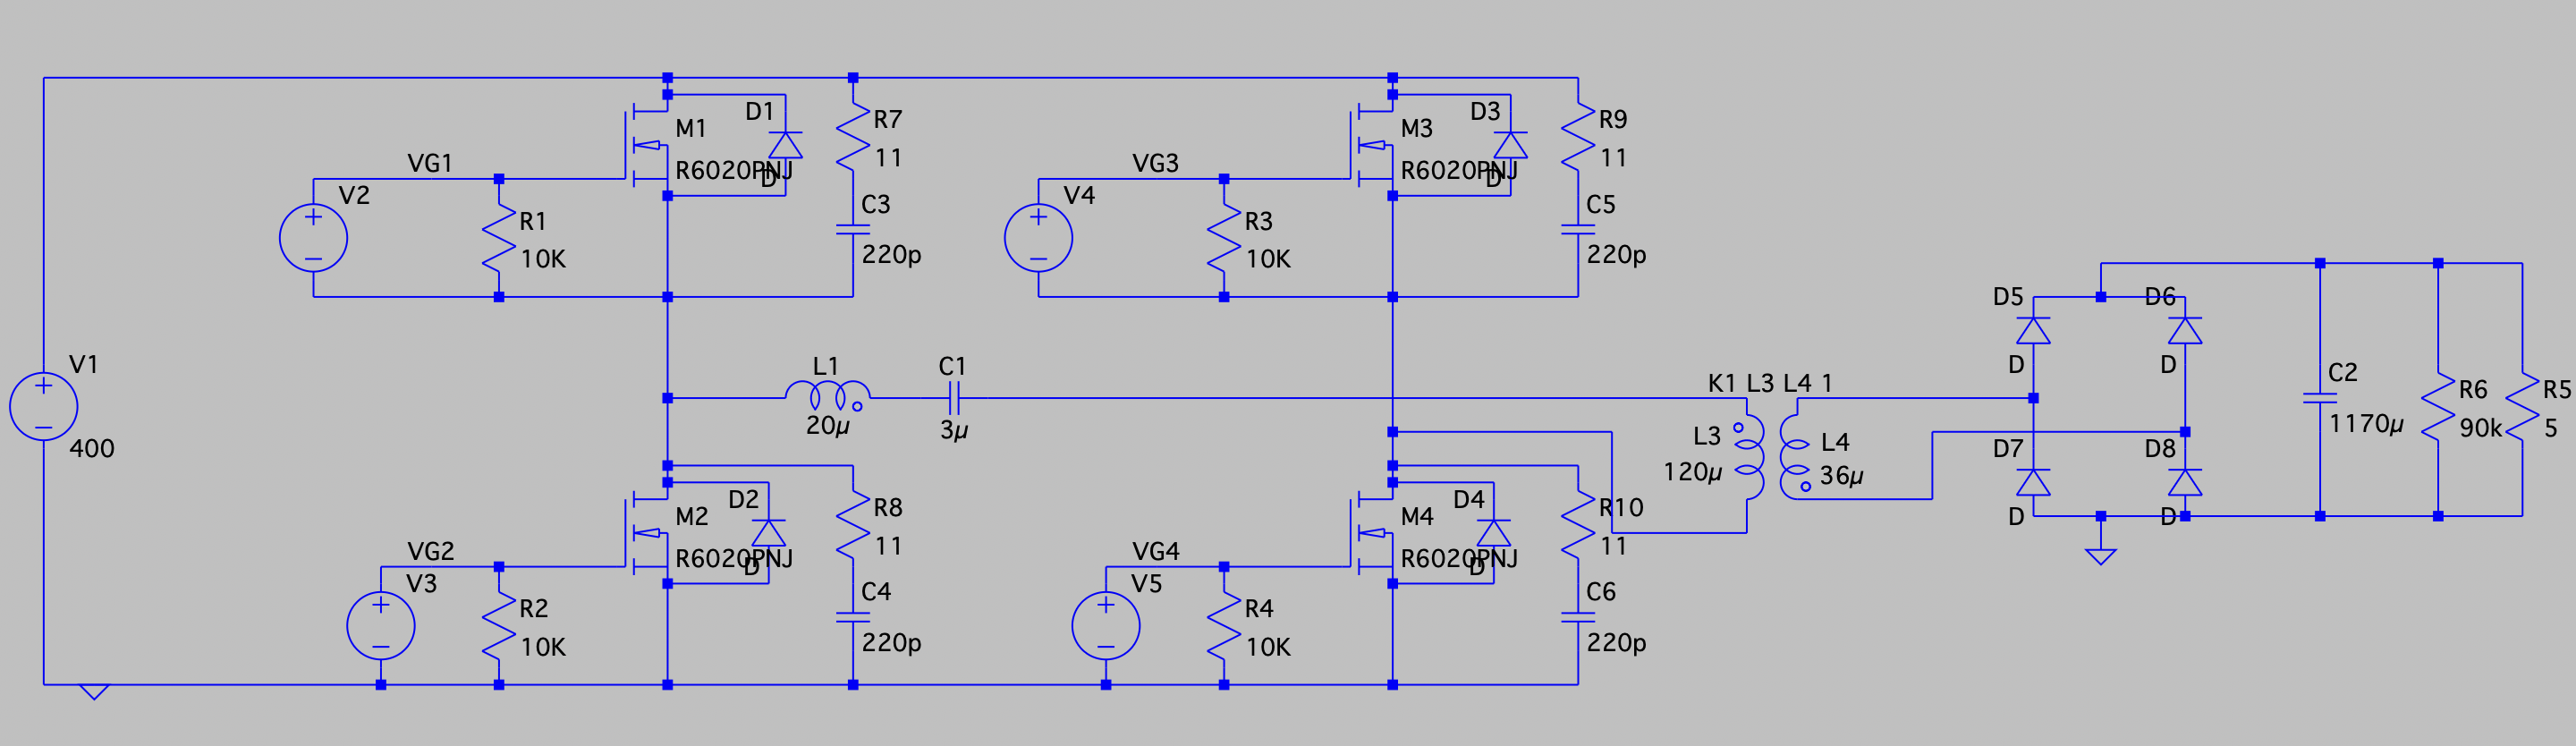
\includegraphics[width=\textwidth]{overall_circuit.png}
    \caption{Simulation}
    \label{fig:Simulation}
\end{figure}
\noindent
Before initiating the design phase, it was imperative to conduct a
comprehensive simulation of the existing design using LtSpice. The simulation
setup (Figure \ref{fig:Simulation}) involved creating the overall circuit as well as the circuits for each
individual sub-sections of the circuit and understanding as well as analyzing
the behavior of each and every sub-circuit.\\
\noindent
The output of the simulation compared with the actual output of each sub-circuit was used to analyze the behavior of the circuit and identify any potential issues that needed to be addressed before proceeding to the design phase.

\subsection{Individual Sectional Simulation}
The complete circuit was divided into multiple sub-sections and each sub-section was simulated individually to understand the behavior of the circuit.

\subsection{Probing Data for Analysis}
The data of each sub-circuit was probed with an oscilloscope and exported as a .csv file to the laptop for analysis.

\subsection{Comparing Oscilloscope Data with Simulation Data}
The simulation data and the probed data were compared against each other to understand the behavior of the circuit and identify any discrepancies.\\
\begin{figure}[H]
    \centering
    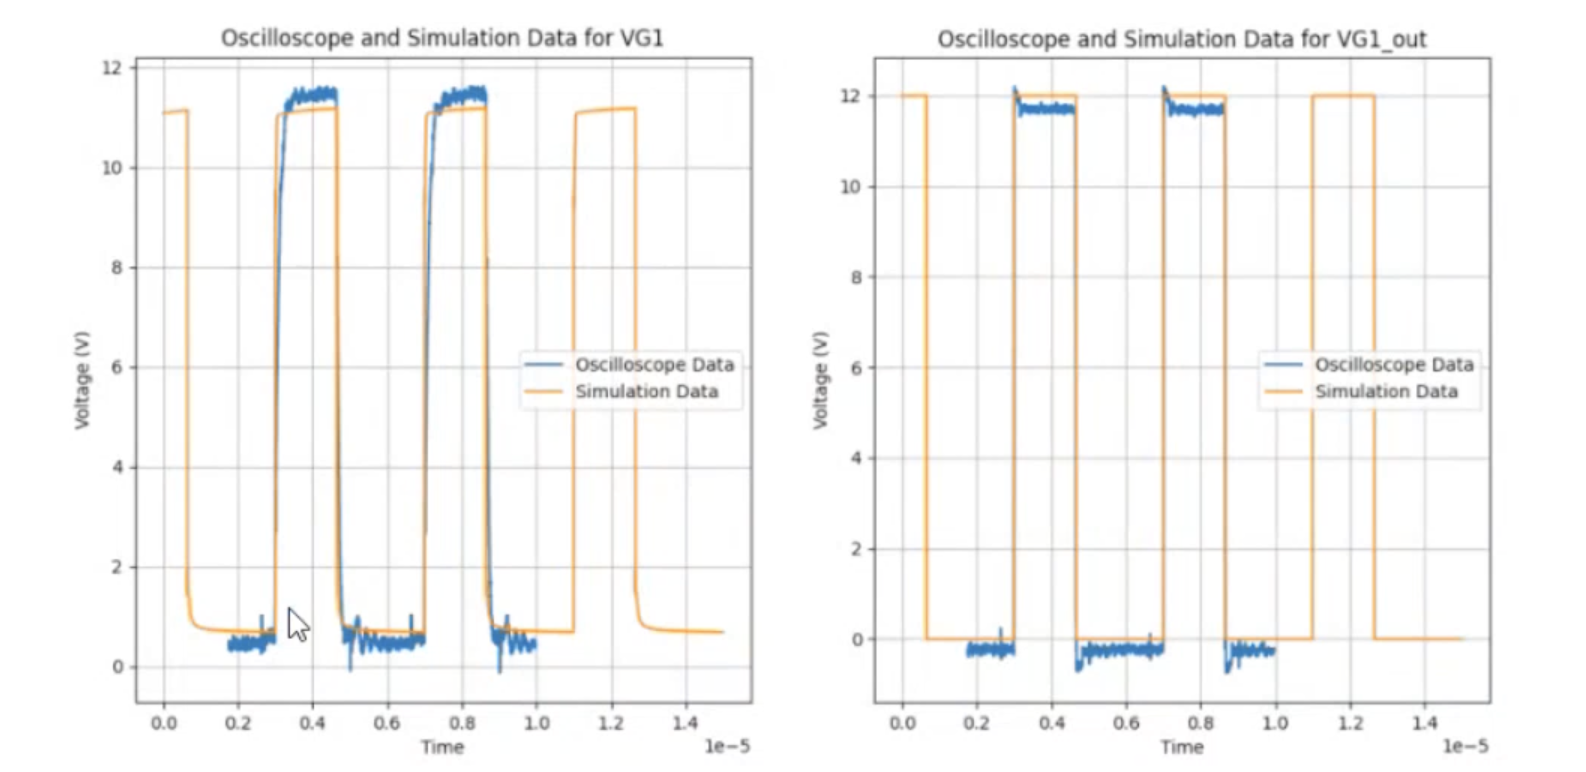
\includegraphics[width=\textwidth]{sectional_output.png}
    \caption{Sectional Output}
    \label{fig:Sectional_Output}
\end{figure}
\noindent
This particular graph (Figure \ref{fig:Sectional_Output}) is of the input and output of the gate driver circuit which is used to pull the gate of the n-channel MOSFEST.

\section{Hardware Testing}
The next step was to get myself involved in the hardware testing of the LLC Converter to know what
all possible issues can arise in the design of such a converter or any potential things that can be
improved from the current design.\\
This helped me learn more about the practical aspects of the design and deepened my understanding of the theoretical concepts.

\subsection{Soldering of the Components}
This involved soldering the components on the PCB and ensuring that the soldering was done properly to avoid any issues during testing.
The soldering was done with lead-free solder to ensure better conductivity and reliable connections.
\subsection{Preparing the Testing Jig of the LLC Converter}
Complete testing procedure was developed which would be used to test the LLC Converter. This involved preparing the testing jig which would be used to test the converter.
This needed to be done carefully to ensure that the testing was done properly and the results were accurate, and the testing jig was efficient in terms for working to ensure high productivity.

\subsection{Debugging Hardware Issues in the Circuit}
Throughout the rest of the internship, I was involved in debugging the hardware issues in the circuit and ensuring that the circuit was working properly.
Multiple issues (such as issue in the feedback signal, issue with the boosting of the voltage, correct mapping of status LEDs to the corresponding pins on the microcontroller) arised during the testing phase which needed to be addressed and resolved to ensure that the circuit was working properly.
The biggest challenge was when we hooked up multiple LLCs in parallel to perform load sharing and we observed oscillications in the load shared. This was solved later by my analysis of the circuit.

\section{Frequency-Gain Curve Plotter for LLC Converters}
Based on the literature that I read during the course of my internship, I made a generalised Frequency-Gain Curve Plotter for the LLC Converter. This plotter would help in understanding the behavior of the converter and would be useful in designing a converter.
\noindent
All we need to do is input our requirements (such as minimum and maximum output voltage, desired resonant frequency, output power) and one or two variables that we choose according to our design and we would get the Frequency-Gain curve for the converter, basically the response of the LLC tank (Gain) for various switching frequencies and then we can tune out the values by optimising the graph as per our requirements.

\section{Design - Calculation of LLC values}
The next step was to design the LLC Converter and calculate the values of the components that would be used in the design. This involved the following steps:

\begin{itemize}
    \item \textbf{Understanding the requirements}: Understanding the requirements of the converter in terms of input and output voltage, current, and power ratings.
    \item \textbf{Selecting the resonant tank components}: Choosing the appropriate resonant tank components to ensure optimal performance and efficiency.
    \item \textbf{Calculating the values of the components}: Calculating the values of the resonant tank components based on the requirements of the converter.
    \item \textbf{Designing the converter}: Designing the converter circuit based on the calculated values of the components.
    \item \textbf{Simulating the converter}: Simulating the converter circuit to verify its performance and efficiency.
    \item \textbf{Optimizing the design}: Optimizing the converter design to maximize efficiency and minimize power losses.
    \item \textbf{Documenting the design}: Documenting the design of the converter to ensure that it can be replicated in the future.
\end{itemize}

\section{Suggestions in current design}
Based on the simulation and analysis of the existing circuit, some changes such as change in the transformer core etc. were suggested in the design to improve the performance and efficiency of the converter. These changes arised by noting that the maximum heat is generated in the transformer only in the current design, so we can improve the efficiency of the current converter as well by changing the transformer core.
The suggested core was PQ40/40 core with PC47 material which has the required power handling capacity, is smaller in terms of footprint, lower EMI noise, and has better efficiency for our operating frequencies. Morever, it is Rs. 70 cheaper than the current core (so if we sell 20,000 units of this power supply, we can save Rs. 14,00,000).

\section{PCB Design}
The last part of my internship included designing the PCB (Figure \ref{fig:pcb_out}) of some other project (RMS - Remote Monitoring System). I used Altium Designer for the same.
\begin{figure}[H]
    \centering
    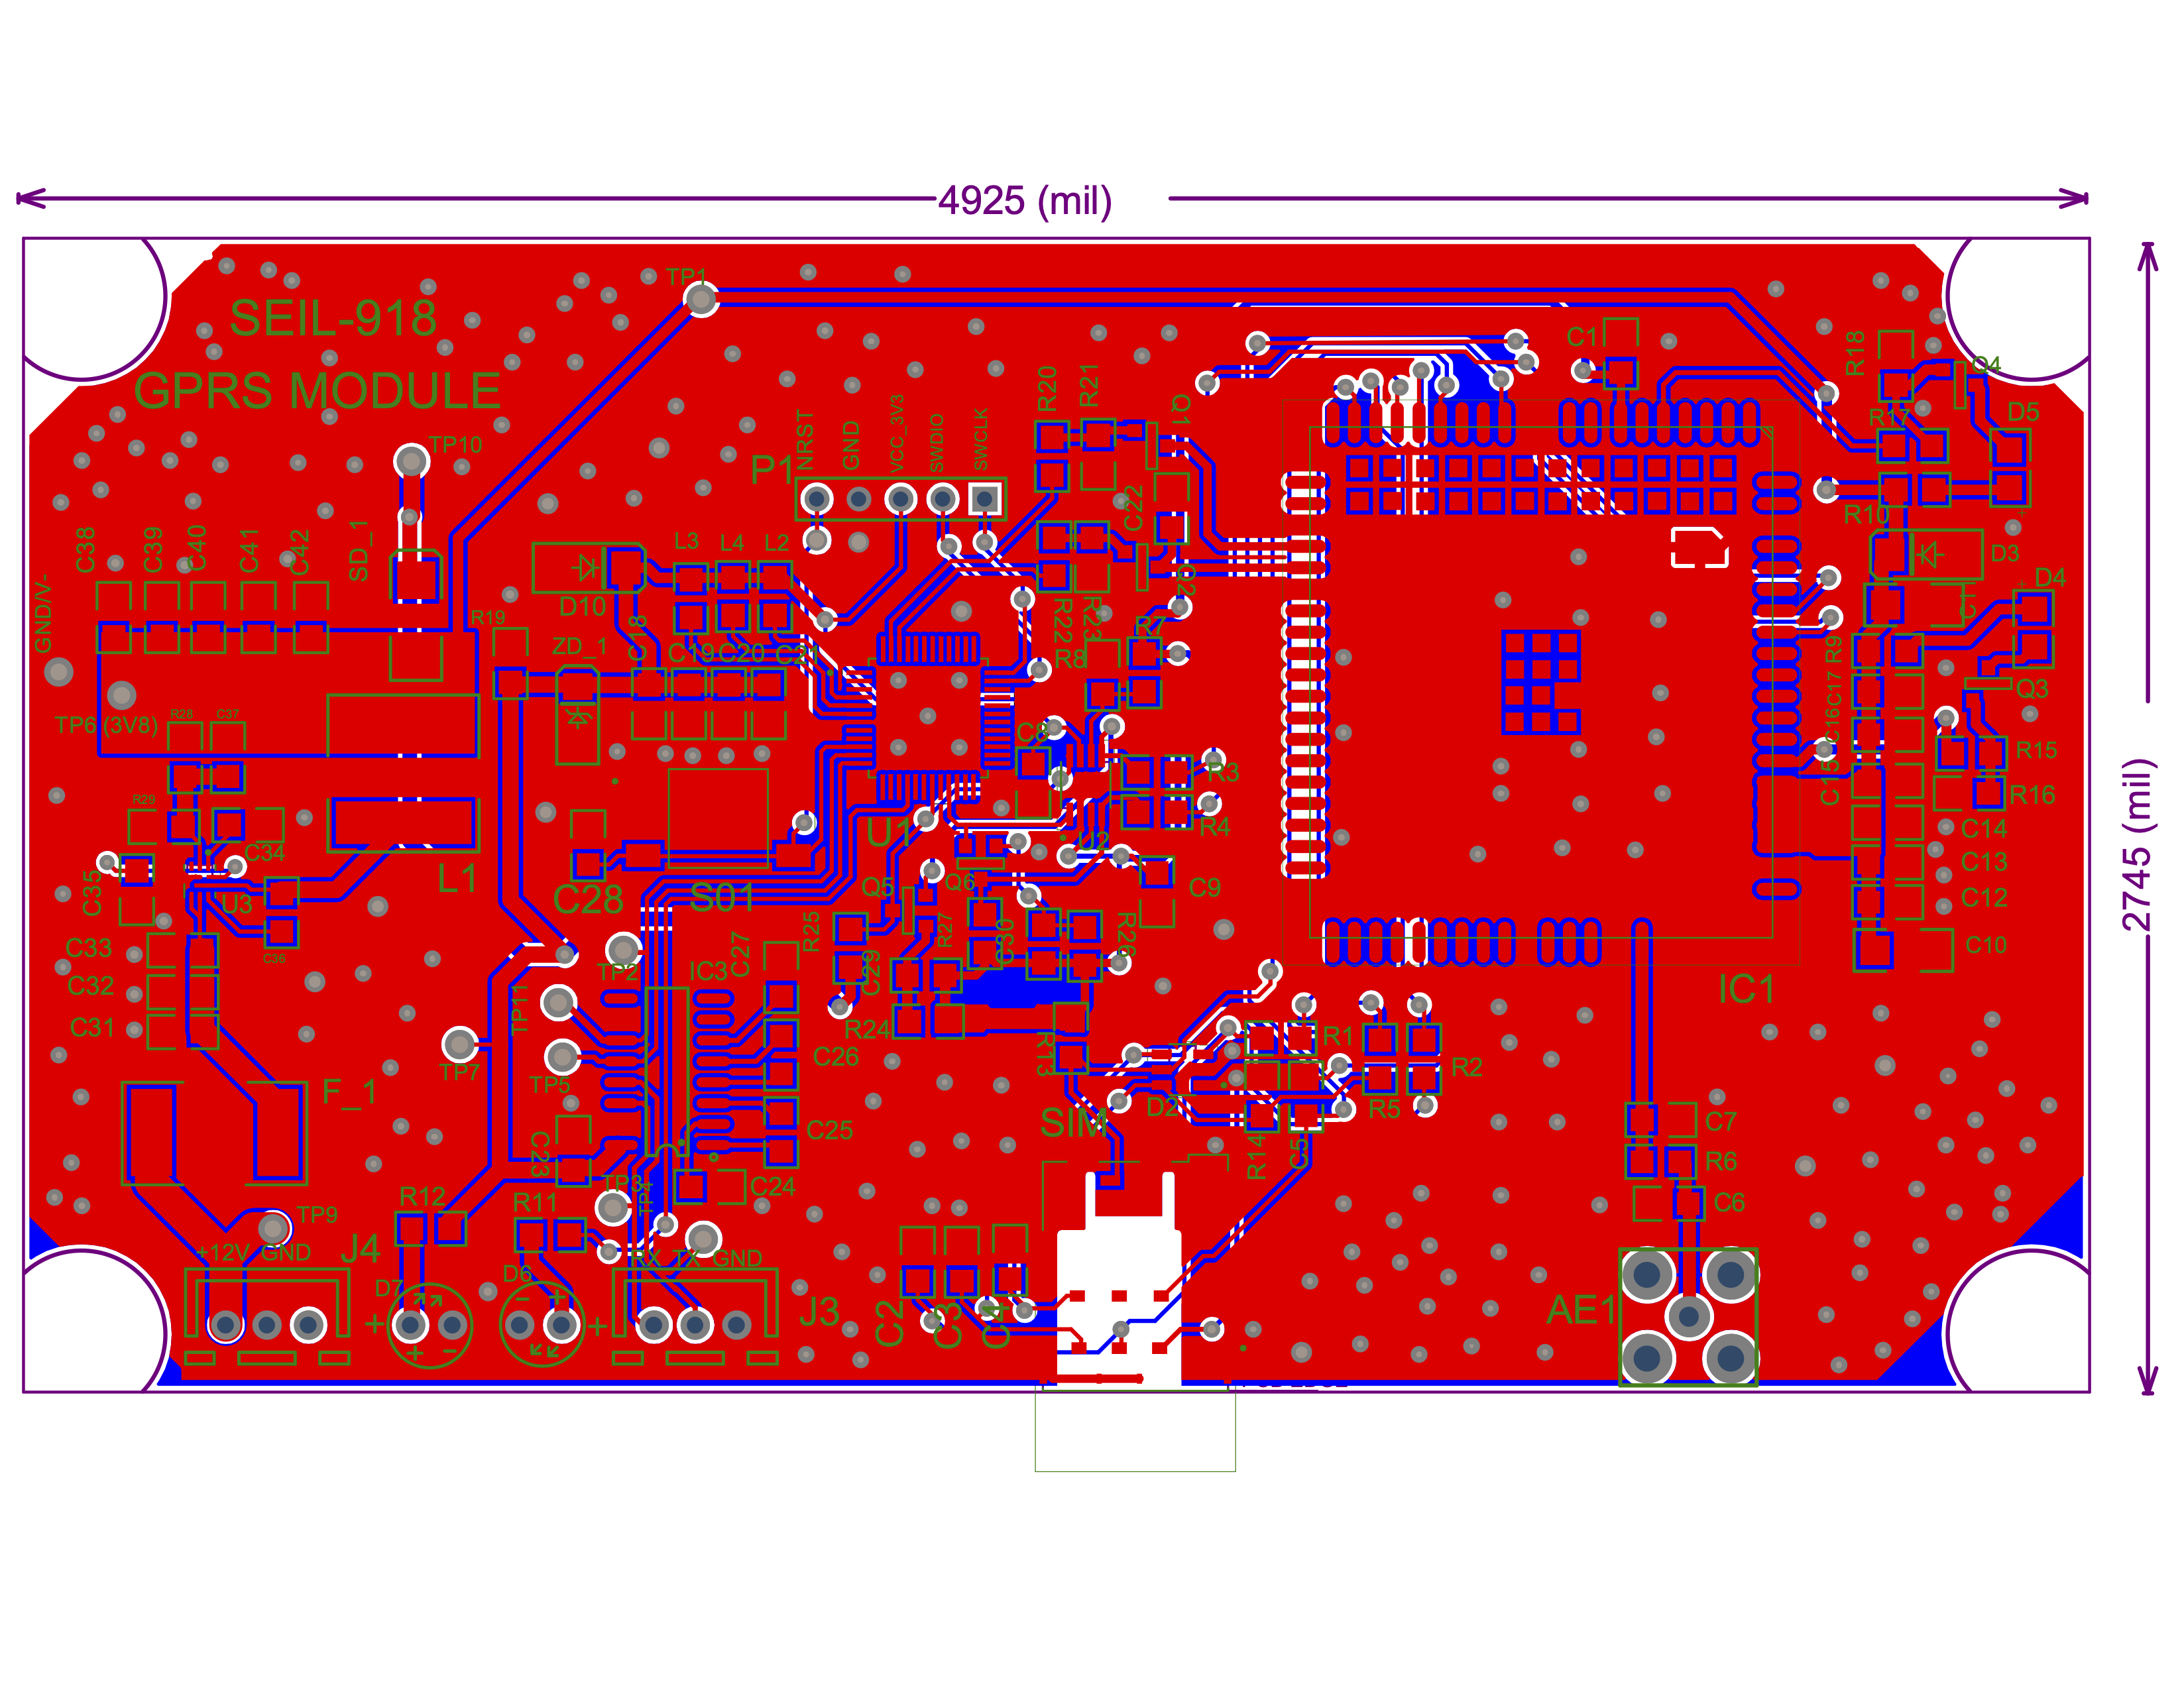
\includegraphics[width=\textwidth]{pcb.png}
    \caption{PCB}
    \label{fig:pcb_out}
\end{figure}